\chapter{Decision Trees}\label{ch-dtree}

\begin{figure}[h!]
\centering
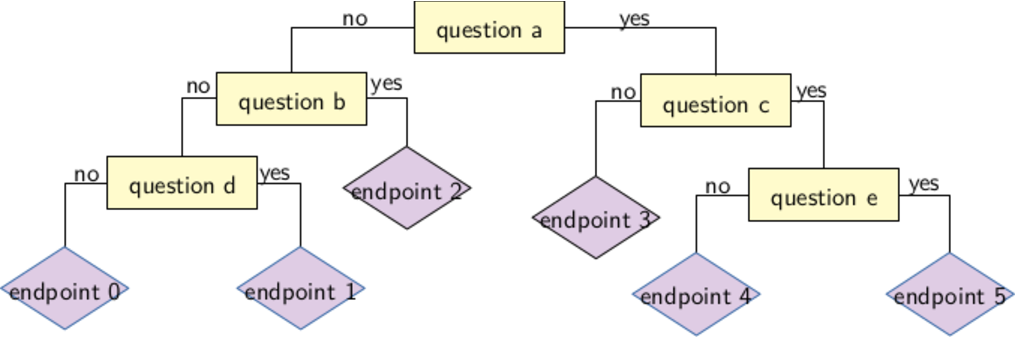
\includegraphics[width=6in]
{dtree/typical-dtree.pdf}
\caption{Typical decision tree.} 
\label{fig-typical-dtree}
\end{figure}

\begin{figure}[h!]
\centering
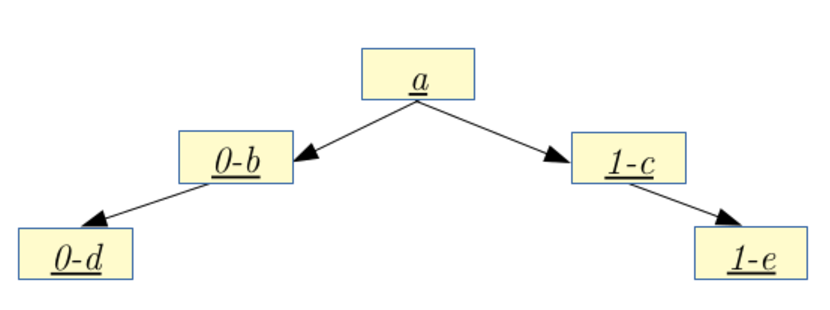
\includegraphics[width=5in]
{dtree/typical-dtree-bnet.pdf}
\caption{Bnet corresponding to 
decision tree
 Fig.\ref{fig-typical-dtree} }
\label{fig-typical-dtree-bnet}
\end{figure}

Fig.\ref{fig-typical-dtree}
shows a typical decision tree (dtree).
The yellow 
rectangles pose 
questions. In general,
the answers to those
questions can
be multiple choices with
more than two choices,
but in Fig.\ref{fig-typical-dtree}
we have chosen the simplest case
of only two choices, 
true or false.
The purple diamonds represent 
endpoints, goals, final
conclusions,
single states of reality, etc.

A trivial 
observation
that is often not made
in dtree educational literature
is that every dtree 
maps into a special bnet, 
let's call it
its ``image" bnet,
in a very natural way.
To get the
 image bnet, just follow the
following simple steps:
\begin{enumerate}
\item {\bf Keep
the yellow question nodes
but reinterpret them as bnet nodes.
Reinterpret the connections among
the dtree question nodes
 as arrows pointing
down from the root node.}

The image bnet nodes
have 3 states,  $0=no$ and
$1=yes$ and $null$.
Table \ref{tab-ternary-trans-prob}
gives the 
node transition matrix $[P(x|a)]_{
x\in \{0,1,null\}, 
a\in \{0,1,null\}}$
where $p_1\in[0,1]$ can be 
different for each node and is given
in the info that specifies    
the dtree. In Table 
\ref{tab-ternary-trans-prob},
$a_0= 0$ if the
dtree node being replaced has input
``no" and $a_0=1$ if its 
input is ``yes".
$!a_0$ means not $a_0$ (i.e., $!a_0=1-a_0$).
\item
{\bf This method of naming
the image bnet nodes
is not necessary but a good practice.}
Give as name to each image bnet
node 
an abridged 
version of
the question
that labels the dtree node it is replacing.
Use as a suffix
to the name of a 
bnet node either a 0 or a 1
depending whether
the dtree node it is replacing
has a 0 or a 1 as input.
This suffix is not
necessary because its
info is already encoded
into
which column
of the node transition prob matrix has 
zero probability for the
$null$ state, but
it's  a redundancy which makes
the bnet easier to read and understand.
\item {\bf Erase the purple endpoint
nodes and connectors to them.} The
info in each  endpoint node
can be preserved
by storing it
as a descriptor (e.g., tool tip)
for the output
states of the
leaf node that 
is the parent
to the endpoint 
in the image bnet.
The
endpoint info can
be added to the descriptor of
the $no=0$ state if the
endpoint has 0 as input 
or to the descriptor
of the $yes=1$ state if 
the endpoint has 1 as input.
\end{enumerate}

% Please add the following required packages to your document preamble:
% \usepackage[table,xcdraw]{xcolor}
% If you use beamer only pass "xcolor=table" option, i.e. \documentclass[xcolor=table]{beamer}
\begin{table}[h!]\centering
\begin{tabular}{|
>{\columncolor[HTML]{ECF4FF}}l |l|l|l|}
\hline
$P(x|a)$ & \cellcolor[HTML]{ECF4FF}$a=a_0$ & \cellcolor[HTML]{ECF4FF}$a=!a_0$ & \cellcolor[HTML]{ECF4FF}$a=null$ \\ \hline
$x=0$    & $1-p_1$                         & 0                                & 0                                \\ \hline
$x=1$    & $p_1$                           & 0                                & 0                                \\ \hline
$x=null$ & 0                               & 1                                & 1                                \\ \hline
\end{tabular}
\caption{Transition probability
matrix of a node
of a dtree image bnet.}
\label{tab-ternary-trans-prob}
\end{table}

Table \ref{tab-node-type}
describes
the node types
commonly used in dtrees.

% Please add the following required packages to your document preamble:
% \usepackage[table,xcdraw]{xcolor}
% If you use beamer only pass "xcolor=table" option, i.e. \documentclass[xcolor=table]{beamer}
\begin{table}[h!]\centering
\begin{tabular}{|l|l|}
\hline
\rowcolor[HTML]{ECF4FF} 
\textbf{\begin{tabular}[c]{@{}l@{}}dtree node types\\ (usual shape in parenthesis)\end{tabular}} & \textbf{\begin{tabular}[c]{@{}l@{}}their node transition probability matrix $P(x|a)$\\  in image bnet\end{tabular}}                               \\ \hline
chance node (oval)                                                                               & $P(x|a)$ arbitrary. random                                                                                                                        \\ \hline
decision node (square)                                                                           & \begin{tabular}[c]{@{}l@{}}$P(x|a)=\delta(x, f(a))$\\ where $f(\cdot)$ is a function of $a$. deterministic\end{tabular}                           \\ \hline
endpoint node (diamond)                                                                          & no $P(x|a)$                                                                                                                                       \\ \hline
fixed node                                                                                       & \begin{tabular}[c]{@{}l@{}}$P(x|a)=\delta(x, x_0)$. $x_0$ does not depend on $a$\\ whereas for decision node it does. deterministic.\end{tabular} \\ \hline
\end{tabular}
\caption{dtree node types. }
\label{tab-node-type}
\end{table}

When drawing dtrees,
some people put
info 
like explanations 
and probabilities on the
connectors 
between the nodes
of  the dtree.
That
info can all
be preserved
in the transition prob matrix
and the descriptors of the
node names and
 node state names
of the image bnet nodes.
Often,
the educational literature
states that 
dtrees are more explicit and  
carry
more info than their
image bnets,
but if one 
follows the above
prescriptions,
both can carry
the same info.

A 
deterministic node
commonly used in dtrees
is one that 
asks
 the question $x<\alpha?$.
for some 
real number
$\alpha\in (L,U)$ and
 some variable $x$ (for
example, $x=$ height of a person).
For such an interval 
splitting  node,
the transition probability
matrix would be as given
in Table \ref{tab-int-split}.
If the interval $[L,U]$
is binned into a number $nbins$
of bins, then
this transition prob matrix will
have dimensions
 ($nbins +1)\times$(
the number of states of the
parent node).


% Please add the following required packages to your document preamble:
% \usepackage[table,xcdraw]{xcolor}
% If you use beamer only pass "xcolor=table" option, i.e. \documentclass[xcolor=table]{beamer}
\begin{table}[h!]\centering
\begin{tabular}{|
>{\columncolor[HTML]{ECF4FF}}l |l|l|l|}
\hline
$P(x|a)$                                        & \cellcolor[HTML]{ECF4FF}\begin{tabular}[c]{@{}l@{}}states of parent node\\ with $a=a_0$\end{tabular} & \cellcolor[HTML]{ECF4FF}\begin{tabular}[c]{@{}l@{}}states of parent node\\ with $a=!a_0$\end{tabular} & \cellcolor[HTML]{ECF4FF}$a=null$ \\ \hline
$[x\in bin]_{\forall\; bin\subset  [L,\alpha)}$ & 1                                                                                                    & 0                                                                                                     & 0                                \\ \hline
$[x\in bin]_{\forall \;bin\subset  [\alpha,U]}$ & 0                                                                                                    & 0                                                                                                     & 0                                \\ \hline
$x=null$                                        & 0                                                                                                    & 1                                                                                                     & 1                                \\ \hline
\end{tabular}
\caption{Transition probability matrix
for interval splitting node.}
\label{tab-int-split}
\end{table}

A naive Bayes bnet 
(see Chapter \ref{ch-naive})
consists of a single ``class"
 node that fans
out with arrows 
pointing to other
``feature" nodes.
If each leaf node
of a naive
Bayes bnet
fans out into 
a set of new leaf
nodes, and those new
leaf nodes
also
fan out
and so on recursively,
we get a 
tree bnet.
The bnet
that arises
from
this recursive
application
of naive Bayes
has the same graph structure
as the image bnet of a dtree.
However, it is more
general because its node
transition prob matrices are more general;
it has more
weights (weight=
parameters of node
transition prob matrices) than a dtree
with the same graph.
